\documentclass[letter]{article}
\renewcommand{\baselinestretch}{1.25}

\usepackage[margin=1in]{geometry}
\usepackage{physics}
\usepackage{amsmath, amsfonts, amssymb, amsthm}
\usepackage{amssymb}
\numberwithin{equation}{section}
\usepackage{amssymb}
\usepackage{graphicx}
\usepackage{hyperref}
\usepackage{empheq}
\usepackage{pdfpages}

% Math Proof things
\newcommand{\Rel}{\mathcal{R}}
\newcommand{\R}{\mathbb{R}}
\newcommand{\C}{\mathbb{C}}
\newcommand{\N}{\mathbb{N}}
\newcommand{\Z}{\mathbb{Z}}
\newcommand{\Q}{\mathbb{Q}}

\newcommand{\st}{\ : \ }

% Theorem Definition
\newtheorem{definition}{Definition}
\newtheorem{assumption}{Assumption}
\newtheorem{theorem}{Theorem}
\newtheorem{lemma}{Lemma}
\newtheorem{proposition}{Proposition}
\newtheorem{example}{Example}

% TikZ Things
\usepackage{tikz}
\usetikzlibrary{positioning,shapes}

% % MATLAB Formatting Code
% \usepackage[numbered,framed]{matlab-prettifier}
% \lstset{style=Matlab-editor,columns=fullflexible}
% \renewcommand{\lstlistingname}{Script}
% \newcommand{\scriptname}{\lstlistingname}

\allowdisplaybreaks

%opening
\title{MECH 6323 - HW 5}
\author{Jonas Wagner}
\date{2022, March 27\textsuperscript{th}}

\begin{document}	

\maketitle

\tableofcontents



% Preliminaries --------------------------------------------
\newpage
\section*{Preliminaries}
\addcontentsline{toc}{section}{Preliminaries}

\begin{definition}
    \textbf{Matrix Basics:} 
    For $A \in \C^{n \cross m}$ and $x \in \C^{m}$,
    \begin{enumerate}
        \item The \emph{\underline{Eigenvalues}} ($\lambda_i$) and \emph{\underline{Eigenvectors}} ($x_i$) of $A$ are defined as the solutions to \[
            \lambda_i A = \lambda_i x_i
        \] 
        \item The \emph{\underline{Spectral Radius}} of $A$ is defined as \[
            \rho(A) := \max_{i} \abs{\lambda_i(A)}
        \]
        \item The \emph{\underline{Complex Conjugate Transpose}} of $A$, denoted as $A^*$, is defined so that \[
            \real(A^*) = \real(A^T)
        \] and \[
            \imaginary(A^*) = - \imaginary(A^T)
        \]
    \end{enumerate}
\end{definition}

\begin{definition}
    \textbf{Vector Norms:} 
    For $x \in \C^{n}$,
    \begin{enumerate}
        \item The \emph{\underline{$2$-norm}}, or \emph{\underline{Euclidean norm}}, is defined as\[
            \norm{x}_2 := \sqrt{\sum_{i=1}^{n} x_{i}^{2}}
        \] 
        \item The \emph{\underline{$1$-norm}} is defined as\[
            \norm{x}_1 := \sum_{i=1}^{n} \abs{x_{i}}
        \] 
        \item The \emph{\underline{$\infty$-norm}} is defined as\[
            \norm{x}_\infty := \max{i = 1,\dots,n} \abs{x_{i}}
        \] 
        \item The \emph{\underline{p-norm}} is defined as\[
            \norm{x}_p := \qty[\sum_{i=1}^{n} \abs{x_{i}}^{p}]^{\frac{1}{p}}
        \]
    \end{enumerate}
\end{definition}

\begin{definition}
    \textbf{Matrix Norms:}
    For $A \in \C^{n \cross m}$ and $x \in \C^{m}$, \begin{enumerate}
        \item The \emph{\underline{Induced $2$-norm}} is defined as \[
            \norm{A}_{2\to2} := \sup_{x \neq 0} \cfrac{\norm{A x}_2}{\norm{x}_2}
        \] and is also known as the \emph{\underline{spectral norm}} and has the additional properties of \begin{enumerate}
            \item $\norm{A}_{2\to2} = \sqrt{\lambda_{max}(A^* A)} = \overline{\sigma}(A)$
            \item $\norm{A^*A}_{2\to2} = \norm{A A^*}_{2\to2} = \norm{A}_2^2$
        \end{enumerate}
    \end{enumerate}
\end{definition}


\begin{definition}
    \textbf{Closed-loop Transfer Functions:} 
    Let $P$ and $C$ represent the plant and controller transfer functions respectively. 
    Within a standard unity feedback system, \begin{enumerate}
        \item the \underline{\emph{sensitivity closed-loop transfer function}} is defined as:\[
            S = \cfrac{1}{1+PC}
        \] 
        \item the \underline{\emph{complementary sensitivity closed-loop transfer function}} is defined as:\[
            T = \cfrac{PC}{1+PC}
        \]
    \end{enumerate}
\end{definition}

\begin{theorem}
    \textbf{Singular Value Decomposition:} 
    Any matrix $M \in \C^{m \cross n}$ can be decomposed as \[
        M = U \Sigma V^*
    \] with $U \in \C^{n \cross n}$ and $V \in \C^{m \cross m}$ are unitary. 
    Additionally, $\Sigma \in \R^{n \cross m}$ was rectangular diagonal with \begin{align*}
        \Sigma = \mqty[
            \hat{\Sigma} &0_{n \cross (m-n)}
        ], \ m \geq n
        &&
        \Sigma = \mqty[
            \hat{\Sigma} \\0_{n \cross (m-n)}
        ], \ n > m
    \end{align*} and \[
        \hat{\Sigma} = \mqty[\dmat{\sigma_1, \sigma_2, \ddots, \sigma_k}] \in \R^{k\cross k}, 
        \quad k = \min(n,m), 
        \quad (\sigma_1 \geq \sigma_2 \geq \cdots \geq 0)
    \] Additionally, $U$ and $V$ are orthonormal, $U U^* = I = V V^*$. \begin{enumerate}
        \item We have \[
            M v_i = \sigma_i u_i
        \] and \[
            M = \sum_{i=1}^{k} \sigma_i u_i v_i^*
        \]
        \item SVD is related to the Eigenvalues and Eigenvectors. \[
            \lambda_i(M^* M) = \sigma_i^2(M)
        \] with corresponding eigenvectors $v_i$ and \[
            \lambda_i(M M^*) = \sigma_i^2(M)
        \] with corresponding eigenvectors $u_i$.
    \end{enumerate}
\end{theorem}

\begin{theorem}
    \textbf{Small-gain Theorem:} 
    Consider an $n_y \cross n_u$ LTI system $M$ and $\Delta \in \C^{n_u \cross n_y}$.
    \begin{figure}[h]
        \centering
        \resizebox*{0.5\textwidth}{!}{
            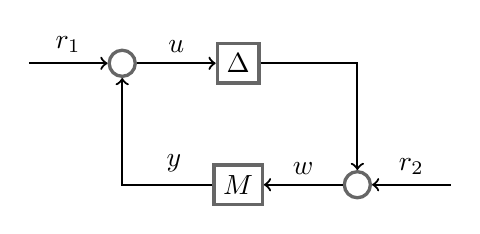
\begin{tikzpicture}[
                block/.style={rectangle, draw=black!60, very thick, minimum size=5mm},
                sum/.style={circle, draw=black!60, very thick, minimum size=2mm},
                empty/.style={coordinate},
                auto
            ]

            %blocks
            \node[block]        (M)                         {$M$};
            \node[block]        (Delta)     [above=of M]    {$\Delta$};

            %sums
            \node[sum]          (in_sum)    [left=of Delta] {};
            \node[sum]          (out_sum)   [right=of M]    {};

            %in/out coordinates
            \node[coordinate]   (in)        [left=of in_sum]    {};
            \node[coordinate]   (out)       [right=of out_sum]  {};

            %arrows
            \draw[->, thick]    (in) -- (in_sum)    node[midway,above] {$r_1$};
            \draw[->, thick]    (out) -- (out_sum)  node[midway,above] {$r_2$};
            \draw[->, thick]    (in_sum) -- (Delta) node[midway,above] {$u$};
            \draw[->, thick]    (out_sum) -- (M)    node[midway,above] {$w$};
            
            %feedback loops
            \draw[->, to path={-| (\tikztotarget)}, thick]
                (M)         edge    (in_sum)
                (Delta)     edge    (out_sum);
            \node[] (y) [left=6mm of M.north] {$y$};

            \end{tikzpicture}
        }
        \caption{Small-gain theorem feedback system}
        \label{fig:small-gain-theorem}
    \end{figure}

    Assuming $M$ is stable, then the feedback system in \figurename \ \ref{fig:small-gain-theorem} is stable for all \ $\overline{\sigma}(\Delta) < m$ if and only if \[
        \norm{M}_\infty \leq \frac{1}{m}
    \]
\end{theorem}







%----- Problem 1 -----------------------------------------------------------------------
\newpage
\section{Problem 1}
Consider the feedback configuration in the figure below.

\begin{figure}[h]
    \centering
    \resizebox*{0.5\textwidth}{!}{
        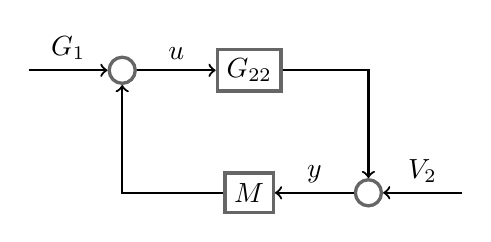
\begin{tikzpicture}[
            block/.style={rectangle, draw=black!60, very thick, minimum size=5mm},
            sum/.style={circle, draw=black!60, very thick, minimum size=2mm},
            empty/.style={coordinate},
            auto
        ]

        %blocks
        \node[block]        (K)                         {$M$};
        \node[block]        (G22)     [above=of K]    {$G_{22}$};

        %sums
        \node[sum]          (in_sum)    [left=of G22] {};
        \node[sum]          (out_sum)   [right=of K]    {};

        %in/out coordinates
        \node[coordinate]   (in)        [left=of in_sum]    {};
        \node[coordinate]   (out)       [right=of out_sum]  {};

        %arrows
        \draw[->, thick]    (in) -- (in_sum)    node[midway,above] {$G_1$};
        \draw[->, thick]    (out) -- (out_sum)  node[midway,above] {$V_2$};
        \draw[->, thick]    (in_sum) -- (G22) node[midway,above] {$u$};
        \draw[->, thick]    (out_sum) -- (K)    node[midway,above] {$y$};
        
        %feedback loops
        \draw[->, to path={-| (\tikztotarget)}, thick]
            (K)         edge    (in_sum)
            (G22)     edge    (out_sum);

        \end{tikzpicture}
    }
    \caption{Problem 1 Feedback Configuration}
    \label{fig:pblm1}
\end{figure}

Prove that\[
    \mqty[
        I       &-K\\
        -G_{22} &I
    ]^{-1}
    = \mqty[
        (I - K G_{22})^{-1}         &(I - K G_{22})^{-1} K\\
        (I - G_{22} K)^{-1} G_22    &(I - G_{22} K)^{-1}
    ]
    = H(G_{22},K)
\]



%----- Problem 2 -----------------------------------------------------------------------
\newpage
\section{Problem 2}
Consider the block diagram in the previous exercise. 
Suppose $G_{22}$ and $K$ have minimal state space realizations $\mqty[
    A   &B_2\\
    C_2 &D_{22}
]$ and $\mqty[
    A_K &B_K\\
    C_K &D_K
]$. Let \[
    T = \mqty[
        A_1 = \mqty[\dmat{A, A_K}]      &B = \mqty[\dmat{B_2, B_k}]\\
        -C = \mqty[0 &-C_K\\ -C_2 & 0]  &D = \mqty[I &-D_K\\ -D_22 &I]
    ]
\] Thus,\[
    T^{-1} = \mqty[
        \overline{A} &\overline{B}\\
        \overline{C} &\overline{D}
    ] := \mqty[
        A_1 + B D^{-1} C    &BD^{-1}\\
        D^{-1} C            &D^{-1}
    ]
\] where \begin{align*}
    \overline{D} = D^{-1} 
    &= \mqty[
            I   &-D_K\\
            -D_{22} &I
        ]^{-1}\\
    &= \mqty[
            I + (I - D_{22} D_K)^{-1} D_{22}    &D_K(I - D_{22} D_K)^{-1}\\
            (I - D_{22}D_K)^{-1}D_22            &(I-D_{22} D_K)^{-1}
        ]\\
    &= \mqty[I &0\\ 0 &0] + \mqty[
            (I - D_{22} D_K)^{-1} D_{22}    &D_K(I - D_{22} D_K)^{-1}\\
            (I - D_{22}D_K)^{-1}D_22            &(I-D_{22} D_K)^{-1}
        ]\\
    &= \mqty[I &0\\ 0 &0] + \mqty[D_K\\I] (I - D_{22} D_K)^{-1} \mqty[D_22 & I]
\end{align*}
Thus,\[
    \overline{A} = A_1 + B D^{-1} C
        = \mqty[
            I &0\\
            0 &0
        ] + \mqty[
            B_2 D_K\\
            B_K
        ] (I - D_{22} D_K)^{-1} \mqty[
            C_2\\
            D_22 C_K
        ]
\]
Prove that the following are equivalent:
\begin{enumerate}
    \item $(\overline{A}, \overline{B}, \overline{C}, \overline{D})$ is stabilizable and detectable.
    \item $(A, B_2, C_2, D_{22})$ and $(A_K, B_K, C_K, D_K)$ are stabilizable and detectable.
\end{enumerate}
















%----- Problem 3 -----------------------------------------------------------------------
\newpage
\section{Problem 3}
For the feedback configuration in \figurename \ \ref{fig:pblm1}, prove that:
\begin{enumerate}
    \item If $K$ is stable then the closed loop interconnection is stable if and only if $G_{22} (I-K G_{22})^{-1}$ is stable.
    \item If $G_{22}$ is stable then the closed loop interconnection is stable if and only if $K (I - G_{22} K)^{-1}$ is stable.
\end{enumerate}






















%----- Problem 4 -----------------------------------------------------------------------
\newpage
\section{Problem 4}
Consider the standard negative feedback loop with the nominal plant dynamics $P(s) = \frac{2}{s+1}$ and controller $K(s) = 20$. 
Assume the ``true'' dynamics lie within the following multiplicative uncertainty set:\[
    \mathcal{M} := \qty{
        \hat{P} = P (1 + W_{u} \Delta) : \norm{\Delta}_\infty < 1 \text{ and } \Delta \text{ stable}
    }
\] Assume the uncertainty weight is $W_{u}(s) = \frac{2s + 1}{s + 10}$.
\begin{enumerate}
    \item Provide an interpretation for the uncertainty describe by the weight $W_u$.
    \item Is the nominal feedback system stable?
    What are the gain and phase margins of the nominal loop $L = PK$?
    \item The robust stability condition for this type of multiplicative uncertainty is stated as: 
    $K$ stabilizes all $\hat{P} \in \mathcal{M}$ if and only if $\norm{W_{u} T}_\infty \leq 1$. 
    Does $K$ robustly stabilize all models in $\mathcal{M}$ based on this condition?
    \item We can construct the uncertainty set M in MATLAB using the following commands:
    \begin{center}
        $>>$ Delta = ultidyn(0Delta0; [1 1]);\\
        $>>$ Phat = P * (1 + Wu * Delta);\\
        $>>$ Lhat = Phat * K;\\
        $>>$ That = feedback(Lhat; 1);
    \end{center}
    The ultidyn command constructs an uncertain, LTI transfer function object that satisfies $\norm{\Delta}_\infty < 1$. 
    The function inputs are the name and input/output size of the object. 
    Construct the uncertain model Phat using the commands above. 
    Generate a Bode magnitude plot with 10 samples drawn from the uncertainty set and draw the nominal response P on the same plot. 
    Note: The command bodemag(Phat) will automatically generate 10 samples and draw their plots.
    \item Finally, we can perform the robustness test using the following command:
    \begin{center}
        $>>$ [stabmarg; destabunc; report] = robstab(That)
    \end{center}
    Refer to the function documentation for robstab for a short description of the input/output arguments. 
    Does the result obtained with robstab agree with your conclusions in part (c)?
\end{enumerate}


















\newpage
\appendix
\section{MATLAB Code:}\label{apx:matlab}
See attached.
Additionally, all the code I write in this course can be found on my GitHub repository:\\
\href{https://github.com/jonaswagner2826/MECH6323}{https://github.com/jonaswagner2826/MECH6323}






\end{document}
